\section{Epipolar Geometry and Stereo Vision}

\begin{itemize}
	\item \textbf{Tie points:} Observed matches across images.
	\item \textbf{Homologous points:} Corresponding projections of the same 3D point.
	\item Both are linked by fundamental matrix (\(\mathbf{F}\)) or essential matrix (\(\mathbf{E}\)) through the epipolar constraint: \(x'^T\mathbf{E}x = 0\)
\end{itemize}
\subsection{Normal Case: 3D Coordinates Computation}
\begin{figure}[ht]
    \centering
    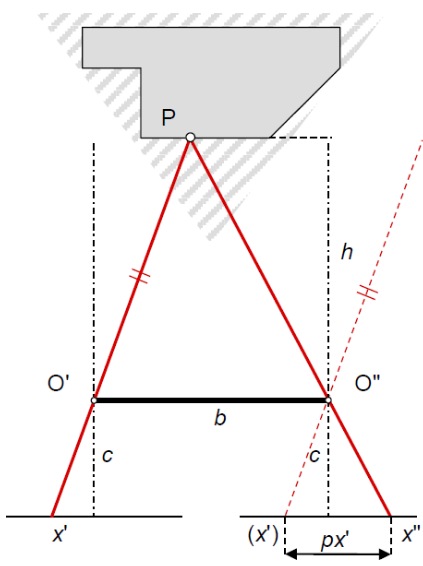
\includegraphics[width = 0.5\columnwidth]{Images/11/normalcase.png}
    \label{fig:normalcase}
\end{figure}
\[
X = \frac{h}{c} \cdot x' = m \cdot x'
\qquad
Y = \frac{h}{c} \cdot y' = m \cdot y'
\]

\[
\frac{h}{c} = \frac{b}{x' - x''} = m
\qquad
Z = h = \frac{b \cdot c}{x' - x''} = \frac{b \cdot c}{p x'}
\]